\section{Motivating example}\label{sec:motivation}
%For the motivating example talk about the case of online memory consumption monitoring.
%Explain how it is useful to perform the monitoring stage of the MAPE Loop.
%Explain the particular case of Component-Based Software Systems built on top of Java (e.g. OSGi, Kevoree)
Online application performance monitoring is a very important concern to detect misbehavior, failures or even potential attacks.
%Self-adaptive and autonomic systems~\cite{kephart2003vision} are systems capable of dynamically adapting their behavior in reponse to changes in their execution environment (failure, performance degradation and so on).
%Self-adaptive systems are generally following a standard architecture called the MAPE-K loop~\cite{Huebscher:2008:SAC:1380584.1380585} which stand for
%Monitoring, Analysis, Planning and Execution.
%Monitoring is the step where the control loop collects meaningful information to drive the system adaptations.
%A self-adaptive system must thus collect data regarding computational resource consumption in order to be resource-aware~\cite{Maheo:2004:MSD:1018420.1019675, Simao:2012:VEJ:2310096.2310158, Guidec:2003:JMP:1899290.1899304}.
At the same time, online memory usage monitoring and analysis is a complex problem when the application development has leveraged specific abstractions. 
This section discusses three motivating examples in which developers use specific abstractions provided by a framework or by himself. 
For each of these examples, we illustrate the mismatch between the concepts used by developers and the concepts manipulated by the state of the art profiling tools. 

Our first example leverage the use of active annotations in the XTend~\cite{bettini2013implementing} language.
Active annotations allow developers to participate in the translation process of Xtend source code to Java code via library.
This is particularly useful when Java requires to write a lot of boilerplate manually. 
For instance, many of the good old design patterns fall into this category. 
An active annotation is an annotation declared either in Java or Xtend, which is itself annotated with Active. 
\textit{@Active} takes a type literal as a parameter pointing to the processor. 
It can be seen as a subset of macro mechanism that exists in Scala or smalltalk~\cite{burmako2013scala}. 
Such mechanism is often used directly by developers to introduce their own abstraction or defining their own internal DSL. 
For example, in the K3-AL\footnote{Available at https://github.com/diverse-project/k3/wiki} project, we use active annotations to create an open-class mechanism in Java~\cite{Clifton:2000:MMO:353171.353181}. 
As a result, the annotation processor change the program structure to implement this feature. 
It adds some methods indirection (to $AASpect$), create new set of objects that represents the state of one conceptual object ($AASpectProperty$), use the Xtend extension method feature, etc\dots 
Figure~\ref{fig:famous} shows the result of this translation process. 
The left part illustrates the code written by the developer, the middle part shows the developer view (the code that can be written to use the open-class mechanism), the right part describes the runtime view. 
 
The current issue is the lack of traceability in the translation process. 
As a result, the abstraction used by the profiler does not match the abstractions used by the developer. 
Adapting profiling tools for these abstractions still requires significant development efforts that must be balanced with the limited audience of these abstractions.

\begin{figure*}
\centering
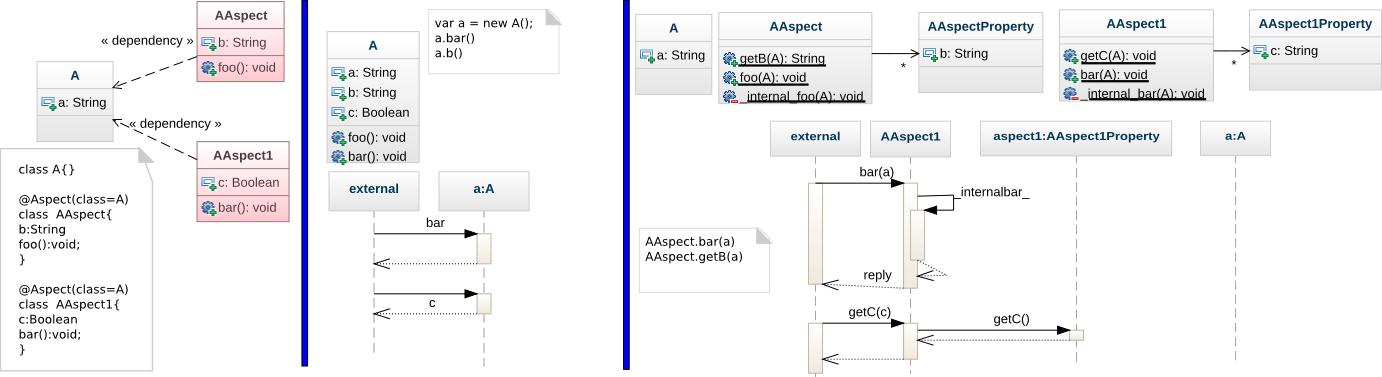
\includegraphics[width=0.9\linewidth]{chapter6/fig/famous}
\caption{Translation process used for building developer abstraction using annotations}
\label{fig:famous}
\end{figure*}

An other example is the OSGi framework. 
In OSGi, developers and users deploy many bundles on top of a single JVM.
It is therefore very complex to decide which bundle should be accounted for the consumption of a particular object because the heap is shared by all the bundles.
A solution to this problem is to account an object $O$ to a bundle if the object $O$ was loaded using the classloader $C$ associated with such a bundle: you can find a path from $C$ to $O$ in the graph of live objects.
This particular solution can be implemented because the mapping between bundle and Java abstractions is known. 
Hence, we can hard-code this mapping in a specific profiler written in JVMTI or we can modify the garbage collector.
Nonetheless, different component-models implementations may map components to different Java abstractions; therefore, the previous solution does not work for all of them.
Thus developers have to design and implement specific profilers from scratch for all the framework and specific abstractions they are using. 
This is a very error prone, hard to debug and time consuming task. 

Finally, the Spring Framework provides a comprehensive programming and configuration model for modern Java-based enterprise applications - on any kind of deployment platform. 
A key element of Spring is its infrastructural support at the application level.
Spring focuses on all the repetitive manual tasks a developer has to handle when developing enterprise applications so that teams can focus on the business logic, without unnecessary ties to specific deployment environments. 
To take care of all these repetitive tasks, Spring provides Dependency Injection, Aspect-Oriented Programming including Spring's declarative transaction management, RESTful web service framework, support for JDBC, JPA, JMS, \dots. 
For all these features, Spring provides abstractions through Java annotations for developers, injects at runtime dynamic proxies to handle these repetitive tasks and adapts the wiring of objects. 
As a result, it exists a mismatch between the running set of objects and the application design. 
This mismatch makes the application profiling difficult and error prone. 
